\documentclass[a4paper, 12pt]{article}

\usepackage[utf8]{inputenc}
\usepackage[T1]{fontenc}
\usepackage{textgreek}
\usepackage{enumitem}
\usepackage{authblk}
\usepackage{graphicx}
\usepackage{float}

\newcommand{\sub}[1]{_{\textup{\scriptsize #1}}}

\title{Summary of TTK4155}
\author{Morten Fyhn Amundsen}
\affil{NTNU}

\begin{document}

\maketitle


An \textbf{embedded system} is an electronic system, consisting of one or more microcontroller which interface with various devices. The system may be part of (\emph{embedded into}) a larger electromechanical system. It is generally designed to perform one specific task, often operating in real time.

Embedded systems are often designed for low power consumption, ruggedness, small size and low per-unit cost.


%%%%%%%%%%%%%%%%%%%%%%%%%%%%%%%%%%%%%%%%%%%%%%%%%%%%%%%%%%%%
\section{Linear voltage regulators}
%%%%%%%%%%%%%%%%%%%%%%%%%%%%%%%%%%%%%%%%%%%%%%%%%%%%%%%%%%%%
\paragraph{Basic linear regulator} Supplies constant voltage with a voltage controlled current source. May need output capacitor to ensure stability. Will have transient error. The pass device is usually made in one of three ways:

\subparagraph{NPN Darlington} Uses Typically gives a voltage drop of $1.5$--$2.2$ V (worst of all types). However, the ground pin current is the lowest (best) of all types. Can supply more current than other types.

\subparagraph{Low-dropout (LDO)} Voltage drop typically $0.6$ V. Best voltage drop, worst ground pin current.

\subparagraph{Quasi-LDO} Somewhere in-between.

\paragraph{Considerations} Max. load current, input voltage source (battery or AC), output voltage tolerance, idle current.



%%%%%%%%%%%%%%%%%%%%%%%%%%%%%%%%%%%%%%%%%%%%%%%%%%%%%%%%%%%%
\section{Switching voltage regulators}
%%%%%%%%%%%%%%%%%%%%%%%%%%%%%%%%%%%%%%%%%%%%%%%%%%%%%%%%%%%%
\paragraph{Buck converter} Down-converts DC. PWM-controls a switch between $V_{in}$ and an inductor-capacitor-path. \textbf{On:} Inductor current to load and capacitor. Capacitor charges. \textbf{Off:} Inductor current to load and back through diode. Capacitor discharges. Cannot completely avoid current ripple. $20$--$30$ \% typical.
\begin{figure}[H]
\centering
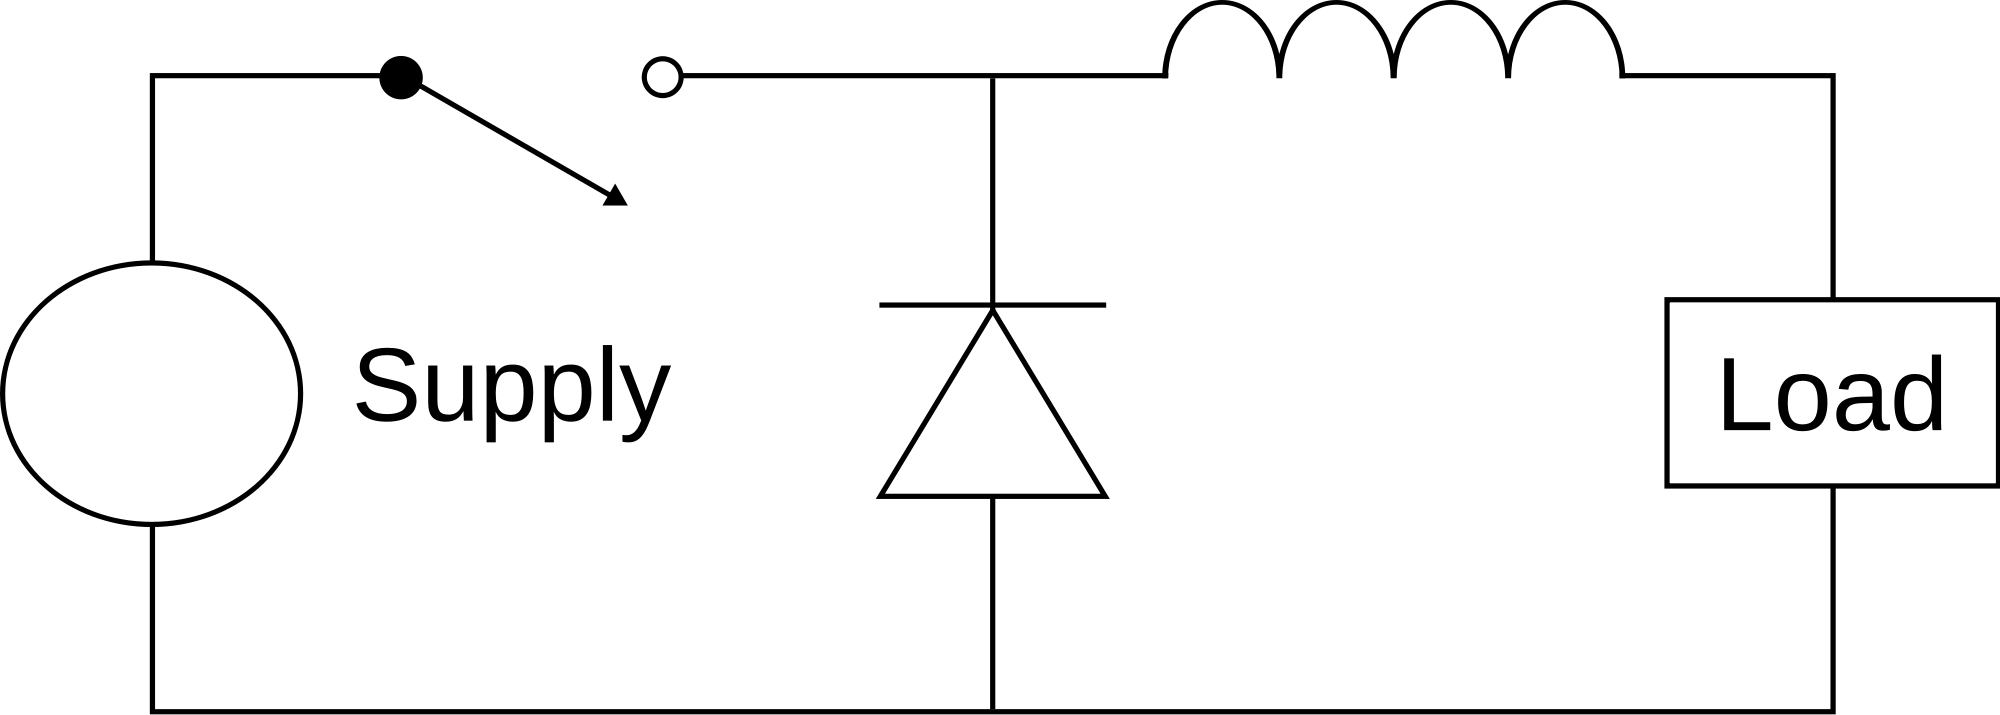
\includegraphics[width=0.5\linewidth]{buck}
\end{figure}

\paragraph{Boost converter} Up-converts DC. \textbf{On:} Inductor shorted to ground, current increases. Load needs capacitor for power. \textbf{Off:} Inductor current must flow through capacitor/load, voltage increases.
\begin{figure}[H]
\centering
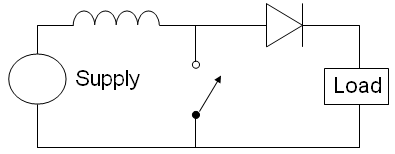
\includegraphics[width=0.5\linewidth]{boost}
\end{figure}

\paragraph{Buck-boost} Gives a DC output of reverse polarity, and either increased or decreased magnitude. \textbf{On:} Capacitor supplies current. \textbf{Off:} Inductor supplies current.

\paragraph{Flyback regulator} Can give several outputs, some of which can be of opposite polarity. It uses transformers with a PWM voltage on the input side, and separate windings for each output.



%%%%%%%%%%%%%%%%%%%%%%%%%%%%%%%%%%%%%%%%%%%%%%%%%%%%%%%%%%%%
\section{CPU}
%%%%%%%%%%%%%%%%%%%%%%%%%%%%%%%%%%%%%%%%%%%%%%%%%%%%%%%%%%%%
\paragraph{RISC}
Reduced instruction set computing. Low number of instruction types. Quick one-cycle execution and pipelining.

\paragraph{Pipelining} Instruction execution partitioned into fixed sequential steps. While one instruction moves to step 2, the next instruction may begin at step 1, i.e. parallell processing.

\subsection{Memory architecture}
\paragraph{Von Neumann} uses the same memory for data and instructions, and cannot fetch both at the same time.
\paragraph{Harvard} uses separate memories with separate buses. Can fetch both at the same time. (Used by ATmega162.)
\paragraph{Hybrid} caches both, but accesses a shared memory in case of cache miss.

\subsection{Memory management}
\paragraph{MMU} is a unit that decodes logical addresses to physical addresses. Must be used for anything except direct-addressed memory (i.e. physical = logical).
\paragraph{Physical memory $>$ logical memory} Divide physical memory into partitions (banks) that are each equal to or less than the logical address space.
\paragraph{Physical memory $<$ logical memory} Exploit the entire logical address space by paging: Load data from secondary storage to physical memory.

%%%%%%%%%%%%%%%%%%%%%%%%%%%%%%%%%%%%%%%%%%%%%%%%%%%%%%%%%%%%
\section{Buses}
%%%%%%%%%%%%%%%%%%%%%%%%%%%%%%%%%%%%%%%%%%%%%%%%%%%%%%%%%%%%
\subsection{Synchronous vs. asynchronous buses}
A synchronous bus has a clock signal sent alongside the data (separate wire). An asynchronous bus does not use a separate clock signal. Instead, the receiver and transmitter must operate at an agreed upon speed, and synchronisation information is sent over the data line(s) periodically to sync their clocks.

\subsection{VMEbus}
32 bit, multi-master, high data transfer rate. Data and address lines can be multiplexed. 7 control lines are used. Runs through a backplane with 1--21 slots for expansion cards. Backplane has a bus controller and some other stuff.

\subsection{PC/104}
An old-ass standard for PC-compatible boards intended for embedded use. The rationale being that using PC hardware and software could greatly decrease R\&D requirements. Units are stackable (like Arduino shields) and smaller than typical PC hardware.

\subsection{I$^2$C}
Two bus lines SDA (data) and SCL (clock), multi-master, 8 bit addressing. Both lines are pulled up.

\subsection{1-Wire}
Only one wire + ground. Supplies data and power (slaves have a half-wave rectifier and a $800$ pF capacitor). Bus is always at $V_{cc}$ when idle, to supply power. Bits are sent as follows:
\begin{itemize}[noitemsep]
\item Logic one: Pull bus low for less than $15$  \textmu s.
\item Logic zero: Low for more than $60$ \textmu s.
\item Bus reset: Low for more than $480$ \textmu s.
\end{itemize}

64 bit serial number fixed to each slave. 48 bits for device address $\rightarrow$ $2^{48} \approx 10^{14}$ addresses $\rightarrow$ no address collisions. (Also 8 bits to tell the type of the device and 8 bit CRC.)

No slave may speak unless requested by the master. No slave--slave communication except through the master.

Communication is initiated by the master resetting the network. Slaves respond with a presence pulse. Master may access any slave through unique addresses.

\subsection{USB}
\paragraph{Topology} Tiered star, i.e. hubs rather than daisy chain. Many devices have built-in hubs. Max. 127 devices per bus.
\paragraph{Bandwidth} USB 3.0: SuperSpeed -- 5 Gbps. USB 2.0: High speed -- 480 Mbps. USB 1.1: Full speed -- 12 Mbps and low speed -- 1.5 Mbps.
\paragraph{Transfer modes} There are four transfer modes.
\subparagraph{Control} Used for command and status operations. Bursty. 8 bit for low speed, 64 bit for full speed, inbetween for high-speed.
\subparagraph{Interrupt} Guaranteed latency transfer, used for HIDs and such. Small amounts of data.
\subparagraph{Bulk} Used for large data amounts. Error detection and correction, guarantee of delivery. Generally fast, but no bandwidth guarantee.
\subparagraph{Isochronous} Guaranteed bandwidth, used for streams and such. Bounded latency. Fault detection, but no retransmission.
\paragraph{Connectors} $V_{bus}$, GND, $D+$, $D-$.

\subsection{U(S)ART}
Universal (Synchronous/)Asynchronous Receiver/Transmitter. A serial communications interface. Sends and receives bits, does not define any protocol. Has, at minimum, TX and RX lines.

\subsection{RS-232}
Defined in 1969, but still useful and common in embedded systems. Defines signals between two devices: Signal names, purpose, voltage levels, connectors and pinouts. Does not define what is sent on the lines. Commonly 1 start bit, 7--9 data bits, 0--1 parity bits, 1--2 stop bits. Only one sender and one receiver per line (usually uses one transmit and one receive line). Is single ended: One line carries signal, one line is common.

\subsection{RS-422}
Faster and more robust than RS-232. Two wires per signal (differential signal). Can connect one transmitter to a bus of up to 10 receivers (almost multidrop).

``Quasi'' multidrop networks can be used: 4 wires, half duplex. Master addresses a node and receives a reply.

\subsection{RS-485}
Up to 32 devices on a data line. Any slave can communicate with any other slave without going via a master. True multi-point network on a single (2 wire) bus. Has clever methods to avoid data collision. Can use more devices if impedance is limited.

\subsection{Controller Area Network}
Two inverse wires, CANL and CANH.
\begin{figure}[H]
\centering
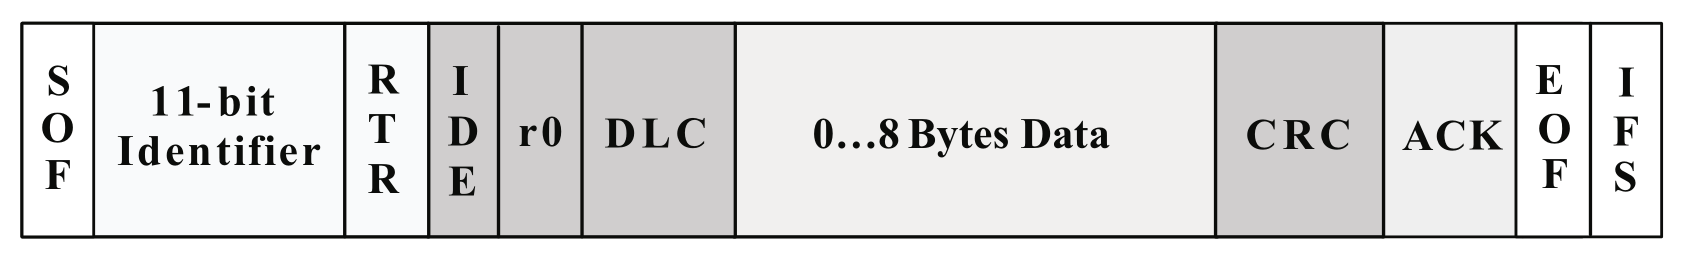
\includegraphics[width=0.8\linewidth]{can_frame}
\end{figure}

\subsubsection{Error detection}
If an error is detected, an error frame is sent. The sender must re-send until the message is sent succesfully. If a node is faulty, e.g. it repeats an error many times, it is deactivated. There are five error tests:
\begin{itemize}[noitemsep]
\item Cyclic redundancy check sent as part of every frame.
\item ACK bits.
\item Form check (check that all bits that must be zero are indeed zero).
\item Each bit it read back by sender and checked.
\item Bit stuffing.
\end{itemize}
\subsubsection{Frame types}
\begin{itemize}[noitemsep]
\item Data frame ---
\item Remote frame ---
\item Error frame ---
\item Overload frame ---
\end{itemize}



%%%%%%%%%%%%%%%%%%%%%%%%%%%%%%%%%%%%%%%%%%%%%%%%%%%%%%%%%%%%
\section{ADC/DAC}
%%%%%%%%%%%%%%%%%%%%%%%%%%%%%%%%%%%%%%%%%%%%%%%%%%%%%%%%%%%%
\subsection{Flash ADC}
With $n$ bit resolution, divides $V\sub{ref}$ into $2^n$ levels (series resistors), compares each level to $V\sub{in}$ with comparators, and calculates the digital value through some logic. Extremely fast, quite expensive to make.
\subsection{Successive approximation ADC}
Compare $V\sub{DAC}$ to $V\sub{in}$. Binary searches through quantisation levels until convergence. (Digital value is run through a DAC for the comparison.)
\subsection{Dual slope ADC} Integrate $V\sub{in}$ for a fixed time. Measure time before integrated value reaches zero again when $-V\sub{ref}$ is connected to input instead of $V\sub{in}$. Doesn't need a sample-and-hold.
\subsection{Types of error}
\paragraph{Static error} Any error found when $V\sub{in}$ is DC.
\paragraph{Quantisation error} $\pm 1/2$ LSB for all ADC types.
\paragraph{Offset error} A nonzero input might give a zero output.
\paragraph{Gain error} The slope of the gain might be slightly off, giving error proportional to voltage.
\paragraph{Differential non-linearity error} Voltage range for each quantisation level might not be of same size for all levels.
\paragraph{Integral non-linearity error} Transition between levels can happen at voltages somewhat offset from the correct voltage.



%%%%%%%%%%%%%%%%%%%%%%%%%%%%%%%%%%%%%%%%%%%%%%%%%%%%%%%%%%%%
\section{Wait states}
%%%%%%%%%%%%%%%%%%%%%%%%%%%%%%%%%%%%%%%%%%%%%%%%%%%%%%%%%%%%
CPU probably faster than peripherals. Injects extra clock cycles into the bus cycle. Makes sure peripherals are read correctly before the next clock cycle.



%%%%%%%%%%%%%%%%%%%%%%%%%%%%%%%%%%%%%%%%%%%%%%%%%%%%%%%%%%%%
\section{Memory management}
%%%%%%%%%%%%%%%%%%%%%%%%%%%%%%%%%%%%%%%%%%%%%%%%%%%%%%%%%%%%

\paragraph{Security} Stop access attempts to reserved memory regions and to memory spaces of other threads (if multithreading). 


\end{document}